% Options for packages loaded elsewhere
\PassOptionsToPackage{unicode}{hyperref}
\PassOptionsToPackage{hyphens}{url}
%
\documentclass[
  11pt,
]{article}
\usepackage[]{mathpazo}
\usepackage{amssymb,amsmath}
\usepackage{ifxetex,ifluatex}
\ifnum 0\ifxetex 1\fi\ifluatex 1\fi=0 % if pdftex
  \usepackage[T1]{fontenc}
  \usepackage[utf8]{inputenc}
  \usepackage{textcomp} % provide euro and other symbols
\else % if luatex or xetex
  \usepackage{unicode-math}
  \defaultfontfeatures{Scale=MatchLowercase}
  \defaultfontfeatures[\rmfamily]{Ligatures=TeX,Scale=1}
  \setmainfont[]{Palatino}
  \setsansfont[]{Helvetica Neue}
  \setmonofont[]{Monaco}
\fi
% Use upquote if available, for straight quotes in verbatim environments
\IfFileExists{upquote.sty}{\usepackage{upquote}}{}
\IfFileExists{microtype.sty}{% use microtype if available
  \usepackage[]{microtype}
  \UseMicrotypeSet[protrusion]{basicmath} % disable protrusion for tt fonts
}{}
\makeatletter
\@ifundefined{KOMAClassName}{% if non-KOMA class
  \IfFileExists{parskip.sty}{%
    \usepackage{parskip}
  }{% else
    \setlength{\parindent}{0pt}
    \setlength{\parskip}{6pt plus 2pt minus 1pt}}
}{% if KOMA class
  \KOMAoptions{parskip=half}}
\makeatother
\usepackage{xcolor}
\IfFileExists{xurl.sty}{\usepackage{xurl}}{} % add URL line breaks if available
\IfFileExists{bookmark.sty}{\usepackage{bookmark}}{\usepackage{hyperref}}
\hypersetup{
  hidelinks,
  pdfcreator={LaTeX via pandoc}}
\urlstyle{same} % disable monospaced font for URLs
\usepackage[margin=1in]{geometry}
\usepackage{color}
\usepackage{fancyvrb}
\newcommand{\VerbBar}{|}
\newcommand{\VERB}{\Verb[commandchars=\\\{\}]}
\DefineVerbatimEnvironment{Highlighting}{Verbatim}{commandchars=\\\{\}}
% Add ',fontsize=\small' for more characters per line
\usepackage{framed}
\definecolor{shadecolor}{RGB}{248,248,248}
\newenvironment{Shaded}{\begin{snugshade}}{\end{snugshade}}
\newcommand{\AlertTok}[1]{\textcolor[rgb]{0.94,0.16,0.16}{#1}}
\newcommand{\AnnotationTok}[1]{\textcolor[rgb]{0.56,0.35,0.01}{\textbf{\textit{#1}}}}
\newcommand{\AttributeTok}[1]{\textcolor[rgb]{0.77,0.63,0.00}{#1}}
\newcommand{\BaseNTok}[1]{\textcolor[rgb]{0.00,0.00,0.81}{#1}}
\newcommand{\BuiltInTok}[1]{#1}
\newcommand{\CharTok}[1]{\textcolor[rgb]{0.31,0.60,0.02}{#1}}
\newcommand{\CommentTok}[1]{\textcolor[rgb]{0.56,0.35,0.01}{\textit{#1}}}
\newcommand{\CommentVarTok}[1]{\textcolor[rgb]{0.56,0.35,0.01}{\textbf{\textit{#1}}}}
\newcommand{\ConstantTok}[1]{\textcolor[rgb]{0.00,0.00,0.00}{#1}}
\newcommand{\ControlFlowTok}[1]{\textcolor[rgb]{0.13,0.29,0.53}{\textbf{#1}}}
\newcommand{\DataTypeTok}[1]{\textcolor[rgb]{0.13,0.29,0.53}{#1}}
\newcommand{\DecValTok}[1]{\textcolor[rgb]{0.00,0.00,0.81}{#1}}
\newcommand{\DocumentationTok}[1]{\textcolor[rgb]{0.56,0.35,0.01}{\textbf{\textit{#1}}}}
\newcommand{\ErrorTok}[1]{\textcolor[rgb]{0.64,0.00,0.00}{\textbf{#1}}}
\newcommand{\ExtensionTok}[1]{#1}
\newcommand{\FloatTok}[1]{\textcolor[rgb]{0.00,0.00,0.81}{#1}}
\newcommand{\FunctionTok}[1]{\textcolor[rgb]{0.00,0.00,0.00}{#1}}
\newcommand{\ImportTok}[1]{#1}
\newcommand{\InformationTok}[1]{\textcolor[rgb]{0.56,0.35,0.01}{\textbf{\textit{#1}}}}
\newcommand{\KeywordTok}[1]{\textcolor[rgb]{0.13,0.29,0.53}{\textbf{#1}}}
\newcommand{\NormalTok}[1]{#1}
\newcommand{\OperatorTok}[1]{\textcolor[rgb]{0.81,0.36,0.00}{\textbf{#1}}}
\newcommand{\OtherTok}[1]{\textcolor[rgb]{0.56,0.35,0.01}{#1}}
\newcommand{\PreprocessorTok}[1]{\textcolor[rgb]{0.56,0.35,0.01}{\textit{#1}}}
\newcommand{\RegionMarkerTok}[1]{#1}
\newcommand{\SpecialCharTok}[1]{\textcolor[rgb]{0.00,0.00,0.00}{#1}}
\newcommand{\SpecialStringTok}[1]{\textcolor[rgb]{0.31,0.60,0.02}{#1}}
\newcommand{\StringTok}[1]{\textcolor[rgb]{0.31,0.60,0.02}{#1}}
\newcommand{\VariableTok}[1]{\textcolor[rgb]{0.00,0.00,0.00}{#1}}
\newcommand{\VerbatimStringTok}[1]{\textcolor[rgb]{0.31,0.60,0.02}{#1}}
\newcommand{\WarningTok}[1]{\textcolor[rgb]{0.56,0.35,0.01}{\textbf{\textit{#1}}}}
\usepackage{graphicx,grffile}
\makeatletter
\def\maxwidth{\ifdim\Gin@nat@width>\linewidth\linewidth\else\Gin@nat@width\fi}
\def\maxheight{\ifdim\Gin@nat@height>\textheight\textheight\else\Gin@nat@height\fi}
\makeatother
% Scale images if necessary, so that they will not overflow the page
% margins by default, and it is still possible to overwrite the defaults
% using explicit options in \includegraphics[width, height, ...]{}
\setkeys{Gin}{width=\maxwidth,height=\maxheight,keepaspectratio}
% Set default figure placement to htbp
\makeatletter
\def\fps@figure{htbp}
\makeatother
\setlength{\emergencystretch}{3em} % prevent overfull lines
\providecommand{\tightlist}{%
  \setlength{\itemsep}{0pt}\setlength{\parskip}{0pt}}
\setcounter{secnumdepth}{-\maxdimen} % remove section numbering
\usepackage{fancyhdr} \setlength{\headheight}{14pt} \usepackage{soul} \usepackage{color} \usepackage{float} \usepackage{hyperref} \usepackage{sectsty} \sectionfont{\centering} \usepackage{enumitem} \usepackage{amsmath} \usepackage{amsfonts} \usepackage{bm} \usepackage{titling} \usepackage[hang,flushmargin]{footmisc} \usepackage{booktabs} \usepackage{lscape}

\title{\fontsize{15pt}{5pt}\selectfont\textbf{Lab Assignment 3}\\
\vspace{.2cm}\textbf{PB HLTH 250C: Advanced Epidemiologic Methods}}
\author{\vspace{-.1cm}\fontsize{15pt}{0pt}\selectfont\textbf{Katherine Rose Wolf}}
\date{\vspace{-.3cm}\fontsize{15pt}{0pt}\selectfont\textbf{\today}}

\begin{document}
\maketitle

\pagebreak

\hypertarget{questions}{%
\section{Questions}\label{questions}}

\hypertarget{question-one}{%
\subsection{Question One}\label{question-one}}

\textbf{Using the R code provided, complete Table 1 using the posterior samples of the odds ratios. \textit{(20 points)}}

\begin{landscape}
\begin{table}
\begin{minipage}{\textwidth}
\caption{Posterior median and 95\% credible intervals for odds ratios from logistic regression model of overweight status on smoking, controlling for age, sex, and education level.}
\begin{tabular}{llll}
\hline
  Variable & Vague prior & Informative Prior 1\footnote{Prior mean for OR of current smoking = 2, prior variance = 1000.} & Informative Prior 2\footnote{Prior mean for OR of current smoking = 2, prior variance = 0.02. (I believe that the prior variance originally listed on the assignment, 0.08, was an error, and that it arose from a given prior interval for Informative Prior 2 of (1, 3), possibly from a prior version of this assignment, instead of (1.5, 2.67). Proof: $(\log(3)-\log(1))/(2*1.96) = 0.079$ whereas $(\log(2.67)-\log(1.5))/(2*1.96) = 0.022$.} \\
  \cline{1-4}
Current smoker (versus not)  & 0.4907 (0.4294, 0.5580) & 0.4879 (0.4299, 0.5552) & 0.6231 (0.5531, 0.7028) \\
Age (per year increase)      & 1.1764 (1.1028, 1.2583) & 1.1784 (1.1007, 1.2571) & 1.2028 (1.1257, 1.2822) \\
Male sex (versus female) & 2.1733 (1.9103, 2.4778) & 2.1812 (1.9086, 2.4832) & 2.0469 (1.7944, 2.3466) \\
High school education (versus < high school education) & 0.6474 (0.5566, 0.7474) & 0.6470 (0.5517, 0.7564) & 0.6462 (0.5545, 0.7544) \\
Some college (versus < high school education) & 0.5339 (0.4442, 0.6434) & 0.5348 (0.4431, 0.6438) & 0.5404 (0.4473, 0.6459) \\
College plus (versus < high school education) & 0.5459 (0.4398, 0.6721) & 0.5439 (0.4411, 0.6744) & 0.5568 (0.4501, 0.6825) \\
\hline
\end{tabular}
\end{minipage}
\end{table}
\end{landscape}

\pagebreak

\hypertarget{question-two}{%
\subsection{Question Two}\label{question-two}}

\textbf{Using the parameterization for Informative Prior 1 (IP1), calculate the prior 95\% interval for the smoking OR. \textit{Hint: Calculate the interval on the scale of the log-OR ($\beta$) and transform the limits.} In \textit{one or two sentences} describe how this compares to the prior interval for Informative Prior 2 (IP2) stated in the instructions above. \textit{(10 points)}}

\textit{Calculations}

Let \(\beta_s\) denote the normal prior for the log odds ratio comparing
the odds (risk) of overweight (body mass index \textgreater{} 25) in a
smoker to that in a nonsmoker. The parameterization for \(\beta_s\)
given for IP1 states that \(\beta_s\) is normally distributed with
hyperparameters mean \(\mu_s\) and variance \(\sigma^2_s\), i.e.,
\(\beta_s \sim N(\mu_s, \sigma^2_s)\), such that the odds ratio
\(e^{\beta_s}\), or the natural exponentiation of the mean of the
log-OR, is 2, i.e., \(e^{E[\beta_s]} = e^{\mu_s} = 2\), and \(\beta_s\)
has a variance of 1000, i.e., \(\sigma^2_s = 1000\).

To get the mean of the log-OR, then, we take the natural logarithm of
the natural exponentiation of the mean of the log-OR, i.e.,
\(\mu_s = \log{e^{\mu_{s}}} = \log(2)\).

To get the standard deviation of \(\beta_s\), \(\sigma_s\), we take the
square root of the variance \(\sigma^2_s\), i.e.,
\(\sigma_s = \sqrt{\sigma^2_s} = \sqrt{1000}\).

Then we can calculate the prior 95\% interval for the log-OR by taking
1.96 standard deviations above and below its mean:

\begin{itemize}
\setlength\itemsep{0em}
\item Lower bound on prior 95\% interval for $\beta_s$: $\mu_s - 1.96\sigma_s = \log(2) - 1.96\sqrt{1000} = -61.287$
\item Upper bound on prior 95\% interval for $\beta_s$: $\mu_s + 1.96\sigma_s = \log(2) + 1.96\sqrt{1000} = 62.674$
\end{itemize}

To get the prior 95\% interval for the OR, \(e^{\beta_s}\), then, we
exponentiate the prior 95\% interval for \(\beta_s\):

\begin{itemize}
\setlength\itemsep{0em}
\item Lower bound on prior 95\% interval for $e^{\beta_s}$: $e^{\mu_s - 1.96\sigma_s} = e^{\log(2) - 1.96\sqrt{1000}} = \ensuremath{2.4165\times 10^{-27}}$
\item Upper bound on prior 95\% interval for $e^{\beta_s}$: $e^{\mu_s + 1.96\sigma_s} = e^{\log(2) + 1.96\sqrt{1000}} = \ensuremath{1.6553\times 10^{27}}$
\end{itemize}

Thus the prior 95\% interval for IP1 is
\((\ensuremath{2.4165\times 10^{-27}}, \ensuremath{1.6553\times 10^{27}})\).

\textit{Comparisons}

The prior 95\% interval drawn from IP1 is
\((\ensuremath{2.4165\times 10^{-27}}, \ensuremath{1.6553\times 10^{27}})\),
corresponding to a variance of 1000, whereas IP2 assumes a prior 95\%
interval of \((1.5, 2.67)\), which, under the assumption of a normal
distribution, yields a variance of only
\((\log(2.67)-\log(1.5))/(2*1.96) = 0.0216\). The drastic difference in
variances determines a drastic difference in the size of the prior
intervals for which we are 95\% confident that we have captured the true
parameter: the wide, flat probability distribution of IP1 assigns almost
equal proabability of the true parameter value appearing among a wide
range of values, whereas IP2's narrow, tall probability distribution
assigns much higher probabilities of the true value appearing the closer
one gets to its mean.

\pagebreak

\hypertarget{question-three}{%
\subsection{Question Three}\label{question-three}}

\textbf{What seems to be more influential on the smoking effect, Informative Prior 1 or Informative Prior 2? In \textit{one sentence}, briefly explain what you think is happening? \textit{(5 points)}}

\textit{Statement}

The model run using IP2 gives an estimate of the posterior median closer
to 2 but a slightly larger confidence interval around it, 0.6231
(0.5531, 0.7028), than the model run using IP1, 0.4879 (0.4299, 0.5552),
showing that IP2 is more influential on the smoking effect than IP1.

\textit{Explanation}

IP2 is more influential because its distribution has a high peak at and
assigns high probabilities to values close to its mean (95\% of the
probability is between 1.5 and 2.67!), which pulls the posterior median
toward it, whereas IP1's much more widely distributed probability
density assigns almost equal probability to the existence of the true
mean anywhere in a big range from \ensuremath{2.4165\times 10^{-27}} to
\ensuremath{1.6553\times 10^{27}}, allowing the new data more latitude
to assign the peak(s) and thus the posterior median.

\pagebreak

\hypertarget{question-four}{%
\subsection{Question Four}\label{question-four}}

\textbf{Using the trace plots, density plots and autocorrelation plots (focus on 1st chain) from the diagnostics for the first model (“Vague prior”), briefly describe any evidence of convergence (or lack of convergence) that you see. Attach these plots (2 pages for trace/density plots; 1 page for autocorrelation plots). \textit{(10 points)}}

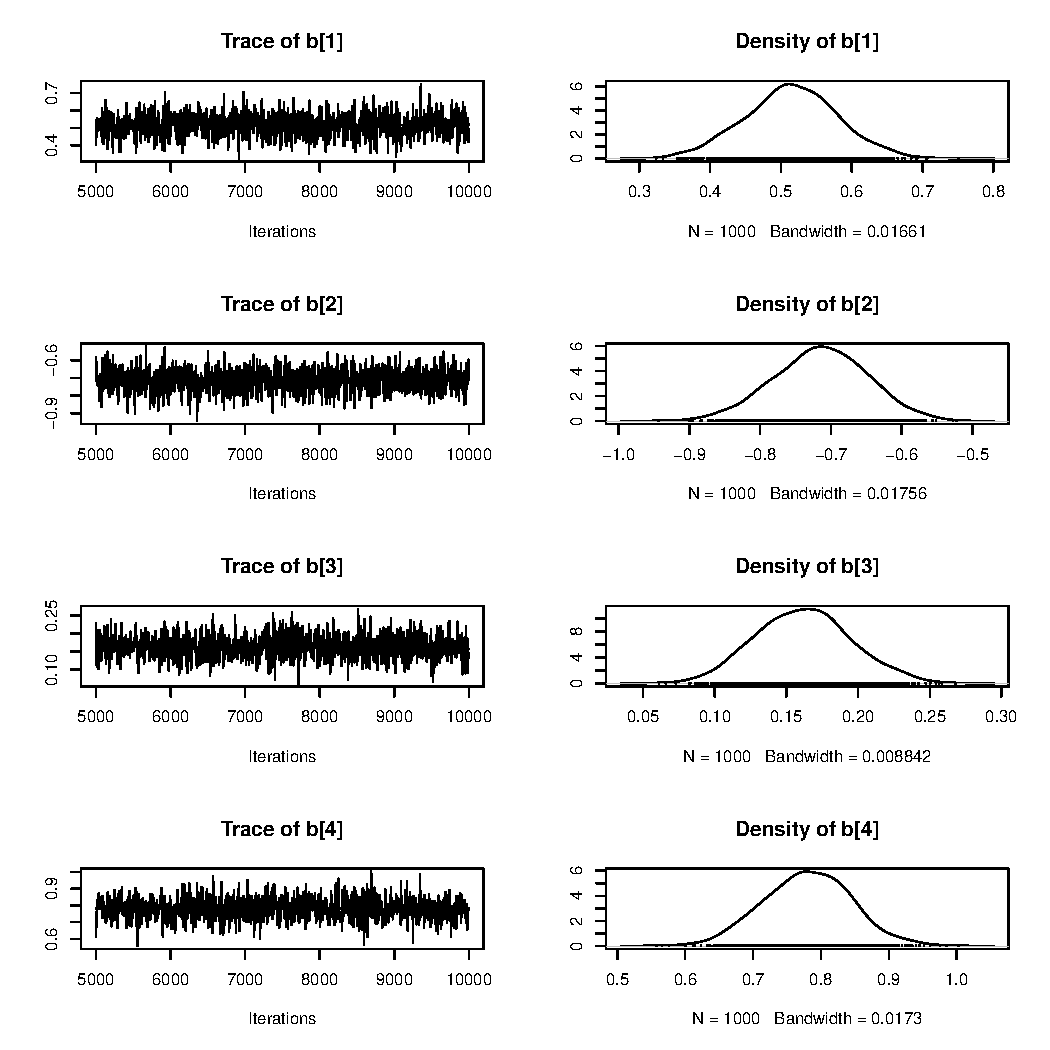
\includegraphics{Traceplot_LogisticReg1.pdf}
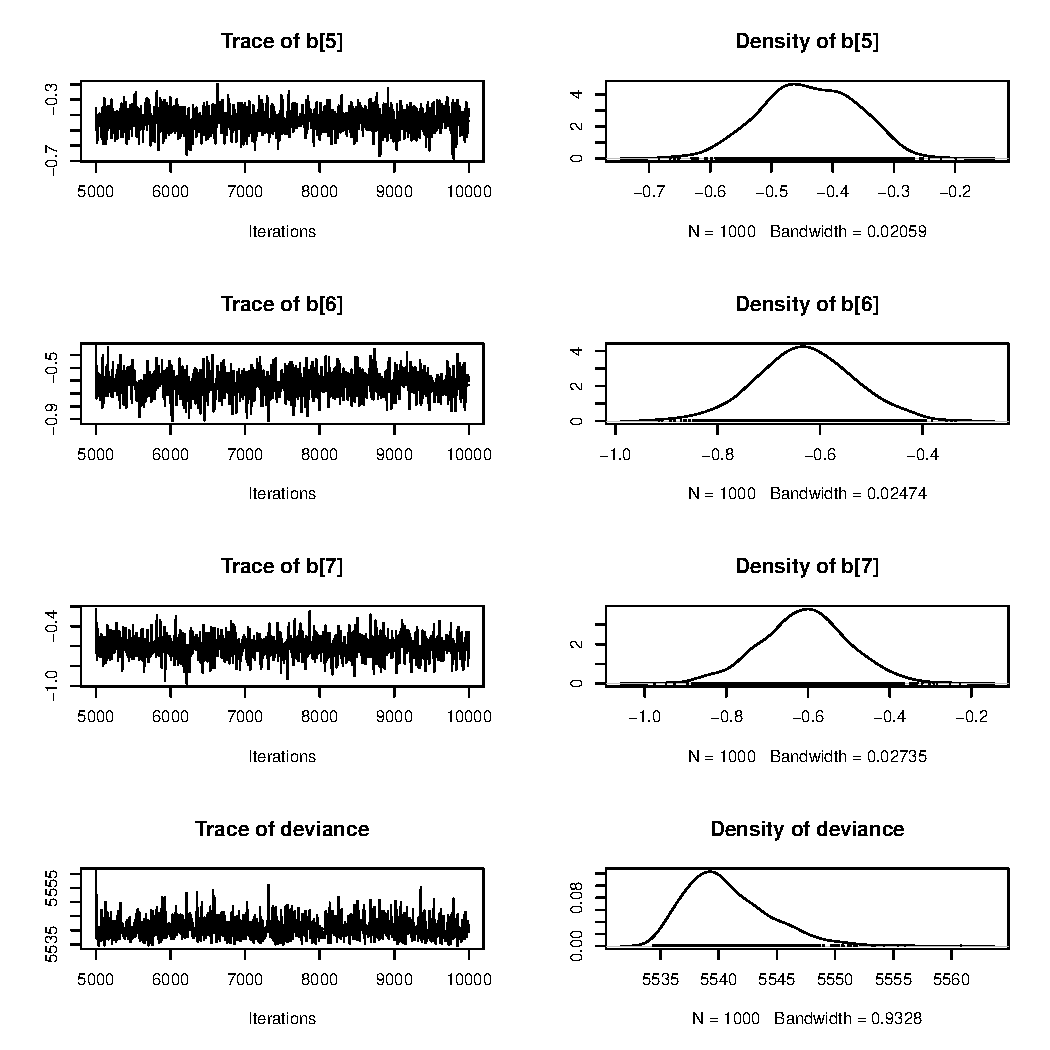
\includegraphics{Traceplot_LogisticReg2.pdf}
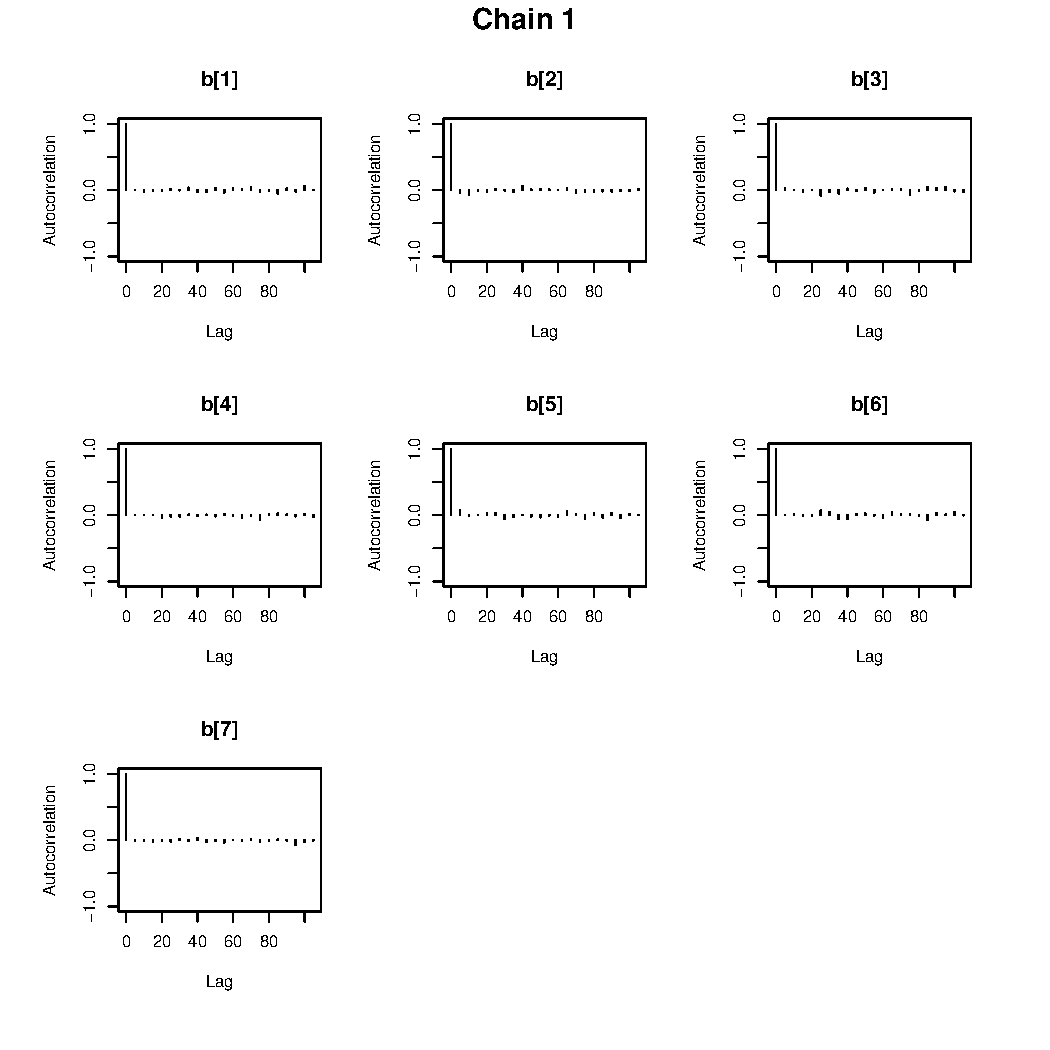
\includegraphics{ACF_LogisticReg.pdf}

\pagebreak

\hypertarget{question-five}{%
\subsection{Question Five}\label{question-five}}

\textbf{From the results of the Geweke test, is there evidence for lack of convergence? Justify your answer. \textit{(5 points)}}

The Geweke test tests whether the Markov Chain is constant between early
and later parts of the sequence of numbers by comparing subsamples of
the random samples for each parameter, here comparing the first 10\% of
the chain to the last half. It outputs the z-statistic and indicates
non-convergence is indicated if the test-statistic is \textgreater{}
1.96 in absolute value.\footnote{Lecture 5, slide 46.}

The Geweke test results here are:

\begin{verbatim}
## [[1]]
## 
## Fraction in 1st window = 0.1
## Fraction in 2nd window = 0.5 
## 
##    b[1]    b[2]    b[3]    b[4]    b[5]    b[6]    b[7] 
## -1.0951  0.1554  0.8022  0.5155 -0.1102  1.1358  1.7095 
## 
## 
## [[2]]
## 
## Fraction in 1st window = 0.1
## Fraction in 2nd window = 0.5 
## 
##    b[1]    b[2]    b[3]    b[4]    b[5]    b[6]    b[7] 
## -1.2630  0.9628  1.0084  0.1967  2.0785  1.7122  1.0630 
## 
## 
## [[3]]
## 
## Fraction in 1st window = 0.1
## Fraction in 2nd window = 0.5 
## 
##    b[1]    b[2]    b[3]    b[4]    b[5]    b[6]    b[7] 
##  0.6734  0.1043  0.3256  0.2065 -0.7789 -1.1426 -1.2885
\end{verbatim}

\pagebreak

\hypertarget{r-code}{%
\section{R code}\label{r-code}}

\begin{Shaded}
\begin{Highlighting}[]
\NormalTok{knitr}\OperatorTok{::}\NormalTok{opts_chunk}\OperatorTok{$}\KeywordTok{set}\NormalTok{(}\DataTypeTok{echo =} \OtherTok{FALSE}\NormalTok{, }
                      \DataTypeTok{warning =} \OtherTok{FALSE}\NormalTok{, }
                      \DataTypeTok{message =} \OtherTok{FALSE}\NormalTok{, }
                      \DataTypeTok{results =} \OtherTok{FALSE}\NormalTok{)}


\KeywordTok{library}\NormalTok{(knitr)}
\KeywordTok{library}\NormalTok{(R2jags)}
\KeywordTok{library}\NormalTok{(coda)}
\KeywordTok{library}\NormalTok{(foreign)}

\KeywordTok{load}\NormalTok{(}\StringTok{"frmgham_recoded_three.Rdata"}\NormalTok{)}


\CommentTok{# Extract data elements from data frame}
\NormalTok{bmi <-}\StringTok{ }\NormalTok{frmgham_recoded}\OperatorTok{$}\NormalTok{bmi}
\NormalTok{overweight <-}\StringTok{ }\KeywordTok{as.integer}\NormalTok{(bmi }\OperatorTok{>=}\StringTok{ }\DecValTok{25}\NormalTok{)}
\NormalTok{cursmoke <-}\StringTok{ }\NormalTok{frmgham_recoded}\OperatorTok{$}\NormalTok{cursmoke}
\NormalTok{age.c <-}\StringTok{ }\KeywordTok{as.numeric}\NormalTok{(}\KeywordTok{scale}\NormalTok{(frmgham_recoded}\OperatorTok{$}\NormalTok{age))}
\NormalTok{male <-}\StringTok{ }\KeywordTok{as.integer}\NormalTok{(frmgham_recoded}\OperatorTok{$}\NormalTok{sex }\OperatorTok{==}\StringTok{ }\DecValTok{1}\NormalTok{)}

\CommentTok{# Create education indicators (a shortcut using the model.matrix command)}
\NormalTok{X.educ <-}\StringTok{ }\KeywordTok{model.matrix}\NormalTok{(}\OperatorTok{~-}\DecValTok{1} \OperatorTok{+}\StringTok{ }\KeywordTok{factor}\NormalTok{(educ), }
                       \DataTypeTok{data=}\NormalTok{frmgham_recoded)}
\NormalTok{educ1 <-}\StringTok{ }\NormalTok{X.educ[,}\DecValTok{1}\NormalTok{]}
\NormalTok{educ2 <-}\StringTok{ }\NormalTok{X.educ[,}\DecValTok{2}\NormalTok{]}
\NormalTok{educ3 <-}\StringTok{ }\NormalTok{X.educ[,}\DecValTok{3}\NormalTok{]}
\NormalTok{educ4 <-}\StringTok{ }\NormalTok{X.educ[,}\DecValTok{4}\NormalTok{]}


\CommentTok{# JAGS code for the posterior distribution:}
\NormalTok{overweight.model <-}\StringTok{ }\ControlFlowTok{function}\NormalTok{() \{}
    \ControlFlowTok{for}\NormalTok{ (i }\ControlFlowTok{in} \DecValTok{1}\OperatorTok{:}\NormalTok{N) \{}
        \KeywordTok{logit}\NormalTok{(pi[i]) <-}\StringTok{ }
\StringTok{            }\NormalTok{b[}\DecValTok{1}\NormalTok{] }\OperatorTok{+}\StringTok{ }
\StringTok{            }\NormalTok{b[}\DecValTok{2}\NormalTok{]}\OperatorTok{*}\NormalTok{cursmoke[i] }\OperatorTok{+}\StringTok{ }
\StringTok{            }\NormalTok{b[}\DecValTok{3}\NormalTok{]}\OperatorTok{*}\NormalTok{age.c[i] }\OperatorTok{+}\StringTok{ }
\StringTok{            }\NormalTok{b[}\DecValTok{4}\NormalTok{]}\OperatorTok{*}\NormalTok{male[i] }\OperatorTok{+}\StringTok{ }
\StringTok{            }\NormalTok{b[}\DecValTok{5}\NormalTok{]}\OperatorTok{*}\NormalTok{educ2[i] }\OperatorTok{+}\StringTok{ }
\StringTok{            }\NormalTok{b[}\DecValTok{6}\NormalTok{]}\OperatorTok{*}\NormalTok{educ3[i] }\OperatorTok{+}\StringTok{ }
\StringTok{            }\NormalTok{b[}\DecValTok{7}\NormalTok{]}\OperatorTok{*}\NormalTok{educ4[i];}
\NormalTok{        overweight[i] }\OperatorTok{~}\StringTok{ }\KeywordTok{dbin}\NormalTok{(pi[i], }\DecValTok{1}\NormalTok{);}
\NormalTok{    \}}
    
\CommentTok{# PRIORS ON BETAS}
\ControlFlowTok{for}\NormalTok{ (j }\ControlFlowTok{in} \DecValTok{1}\OperatorTok{:}\NormalTok{Nx)\{}
\NormalTok{    b[j] }\OperatorTok{~}\StringTok{ }\KeywordTok{dnorm}\NormalTok{(mu[j], }
\NormalTok{                 tau[j]); }\CommentTok{# Independent normal priors}
\NormalTok{    OR[j] <-}\StringTok{ }\KeywordTok{exp}\NormalTok{(b[j]); }\CommentTok{# Calculate the odds ratios}
\NormalTok{    \}}
\NormalTok{\}}


\CommentTok{# constants to be passed in}
\NormalTok{N <-}\StringTok{ }\KeywordTok{length}\NormalTok{(overweight); }\CommentTok{# number of observations to loop over}
\NormalTok{Nx <-}\StringTok{ }\DecValTok{7}\NormalTok{; }\CommentTok{# number of parameters (w/ intercept)}
\NormalTok{n.iter <-}\StringTok{ }\DecValTok{10000}\NormalTok{; }\CommentTok{# number of iterations to run (total)}

\CommentTok{# Parameters on the priors:}
\NormalTok{mu <-}\StringTok{ }\KeywordTok{rep}\NormalTok{(}\DecValTok{0}\NormalTok{,Nx); }\CommentTok{# Prior mean of betas}
\NormalTok{tau <-}\StringTok{ }\KeywordTok{rep}\NormalTok{(.}\DecValTok{001}\NormalTok{,Nx); }\CommentTok{# Prior precisions}

\CommentTok{# List of data elements to pass in:}
\NormalTok{overweight.data <-}\StringTok{ }\KeywordTok{list}\NormalTok{(}\StringTok{"N"}\NormalTok{, }
                        \StringTok{"Nx"}\NormalTok{, }
                        \StringTok{"overweight"}\NormalTok{, }
                        \StringTok{"age.c"}\NormalTok{, }
                        \StringTok{"male"}\NormalTok{, }
                        \StringTok{"cursmoke"}\NormalTok{,}
                        \StringTok{"educ2"}\NormalTok{, }
                        \StringTok{"educ3"}\NormalTok{,}
                        \StringTok{"educ4"}\NormalTok{,}
                        \StringTok{"mu"}\NormalTok{,}
                        \StringTok{"tau"}\NormalTok{)}

\CommentTok{# List of parameters to keep track of:}
\NormalTok{overweight.parameters <-}\StringTok{ }\KeywordTok{c}\NormalTok{(}\StringTok{"b"}\NormalTok{, }\StringTok{"OR"}\NormalTok{)}

\CommentTok{# Function to generate initial values for each chain:}
\NormalTok{overweight.inits <-}\StringTok{ }\ControlFlowTok{function}\NormalTok{() \{}\KeywordTok{list}\NormalTok{ (}\DataTypeTok{b =} \KeywordTok{rnorm}\NormalTok{(Nx, }\DecValTok{0}\NormalTok{ , }\DataTypeTok{sd =} \FloatTok{0.5}\NormalTok{))\}}


\KeywordTok{set.seed}\NormalTok{(}\DecValTok{123}\NormalTok{)}
\NormalTok{overweight.sim <-}\StringTok{ }\KeywordTok{jags}\NormalTok{(}\DataTypeTok{data =}\NormalTok{ overweight.data,}
                       \DataTypeTok{model.file =}\NormalTok{ overweight.model,}
                       \DataTypeTok{inits =}\NormalTok{ overweight.inits,}
                       \DataTypeTok{parameters.to.save =}\NormalTok{ overweight.parameters,}
                       \DataTypeTok{n.iter =}\NormalTok{ n.iter)}

\KeywordTok{print}\NormalTok{(overweight.sim, }\DataTypeTok{digits =} \DecValTok{4}\NormalTok{)}


\NormalTok{overweight.mcmc <-}\StringTok{ }\KeywordTok{as.mcmc}\NormalTok{(overweight.sim)}

\CommentTok{# Traceplot and density plots for regression coefficients}
\CommentTok{# code will save to PDF in current directory.}
\CommentTok{# Execute "plot" commands only to plot to screen.}
\KeywordTok{pdf}\NormalTok{(}\StringTok{"Traceplot_LogisticReg1.pdf"}\NormalTok{) }\CommentTok{# Write what comes next to PDF file}
\KeywordTok{plot}\NormalTok{(overweight.mcmc[}\DecValTok{1}\NormalTok{][, }\DecValTok{1}\OperatorTok{:}\DecValTok{4}\NormalTok{]) }\CommentTok{# For beta1-4}

\KeywordTok{pdf}\NormalTok{(}\StringTok{"Traceplot_LogisticReg2.pdf"}\NormalTok{) }\CommentTok{# Write what comes next to PDF file}
\KeywordTok{plot}\NormalTok{(overweight.mcmc[}\DecValTok{1}\NormalTok{][, }\DecValTok{5}\OperatorTok{:}\DecValTok{8}\NormalTok{]) }\CommentTok{# For beta5-7 and deviance}

\KeywordTok{dev.off}\NormalTok{() }\CommentTok{# Stop writing to the PDF file}

\CommentTok{# Autocorrelation plots for the regression coefficients}
\KeywordTok{pdf}\NormalTok{(}\StringTok{"ACF_LogisticReg.pdf"}\NormalTok{)}
\KeywordTok{par}\NormalTok{(}\DataTypeTok{omi=}\KeywordTok{c}\NormalTok{(.}\DecValTok{25}\NormalTok{, }\FloatTok{.25}\NormalTok{, }\FloatTok{.25}\NormalTok{, }\FloatTok{.25}\NormalTok{)) }\CommentTok{# Create an outer margin (room for title)}

\KeywordTok{autocorr.plot}\NormalTok{(overweight.mcmc[}\DecValTok{1}\NormalTok{][, }\DecValTok{1}\OperatorTok{:}\DecValTok{7}\NormalTok{]) }\CommentTok{# For chain 1}
\KeywordTok{title}\NormalTok{(}\StringTok{"Chain 1"}\NormalTok{, }\DataTypeTok{outer=}\NormalTok{T) }\CommentTok{# Place title in outer margin of page}

\KeywordTok{autocorr.plot}\NormalTok{(overweight.mcmc[}\DecValTok{2}\NormalTok{][, }\DecValTok{1}\OperatorTok{:}\DecValTok{7}\NormalTok{]) }\CommentTok{# For chain 2 (optional)}
\KeywordTok{title}\NormalTok{(}\StringTok{"Chain 2"}\NormalTok{, }\DataTypeTok{outer=}\NormalTok{T)}

\KeywordTok{autocorr.plot}\NormalTok{(overweight.mcmc[}\DecValTok{3}\NormalTok{][, }\DecValTok{1}\OperatorTok{:}\DecValTok{7}\NormalTok{]) }\CommentTok{# For chain 3 (optional)}
\KeywordTok{title}\NormalTok{(}\StringTok{"Chain 3"}\NormalTok{, }\DataTypeTok{outer=}\NormalTok{T)}

\KeywordTok{dev.off}\NormalTok{()}

\KeywordTok{geweke.diag}\NormalTok{(overweight.mcmc[,}\DecValTok{1}\OperatorTok{:}\DecValTok{7}\NormalTok{]) }\CommentTok{# Geweke test}


\CommentTok{# Informative prior 1 (Change prior mean to log(2) for b[2])}
\NormalTok{mu[}\DecValTok{2}\NormalTok{] <-}\StringTok{ }\KeywordTok{log}\NormalTok{(}\DecValTok{2}\NormalTok{)}

\KeywordTok{set.seed}\NormalTok{(}\DecValTok{123}\NormalTok{)}
\NormalTok{overweight.sim.inform1 <-}\StringTok{ }\KeywordTok{jags}\NormalTok{(}\DataTypeTok{data =}\NormalTok{ overweight.data,}
                               \DataTypeTok{model.file =}\NormalTok{ overweight.model,}
                               \DataTypeTok{inits =}\NormalTok{ overweight.inits,}
                               \DataTypeTok{parameters.to.save =}\NormalTok{ overweight.parameters,}
                               \DataTypeTok{n.iter =}\NormalTok{ n.iter)}

\KeywordTok{print}\NormalTok{(overweight.sim.inform1, }\DataTypeTok{digits =} \DecValTok{4}\NormalTok{)}


\CommentTok{# Informative prior 2 (Change prior precision to 1/0.1225 vor beta[4])}
\NormalTok{sd.prior <-}\StringTok{ }\NormalTok{(}\KeywordTok{log}\NormalTok{(}\FloatTok{2.67}\NormalTok{) }\OperatorTok{-}\StringTok{ }\KeywordTok{log}\NormalTok{(}\FloatTok{1.5}\NormalTok{))}\OperatorTok{/}\NormalTok{(}\DecValTok{2}\OperatorTok{*}\FloatTok{1.96}\NormalTok{) }\CommentTok{# SD for beta2 on log-scale}
\NormalTok{tau[}\DecValTok{2}\NormalTok{] <-}\StringTok{ }\DecValTok{1}\OperatorTok{/}\NormalTok{sd.prior}\OperatorTok{^}\DecValTok{2} \CommentTok{# Convert to precision (reciprocal of variance)}

\KeywordTok{set.seed}\NormalTok{(}\DecValTok{123}\NormalTok{)}

\NormalTok{overweight.sim.inform2 <-}\StringTok{ }\KeywordTok{jags}\NormalTok{(}\DataTypeTok{data =}\NormalTok{ overweight.data,}
                               \DataTypeTok{model.file =}\NormalTok{ overweight.model,}
                               \DataTypeTok{inits =}\NormalTok{ overweight.inits,}
                               \DataTypeTok{parameters.to.save =}\NormalTok{ overweight.parameters,}
                               \DataTypeTok{n.iter =}\NormalTok{ n.iter)}

\KeywordTok{print}\NormalTok{(overweight.sim.inform2, }\DataTypeTok{digits=}\DecValTok{4}\NormalTok{)}

            \CommentTok{# b[1] + }
            \CommentTok{# b[2]*cursmoke[i] + }
            \CommentTok{# b[3]*age.c[i] + }
            \CommentTok{# b[4]*male[i] + }
            \CommentTok{# b[5]*educ2[i] + }
            \CommentTok{# b[6]*educ3[i] + }
            \CommentTok{# b[7]*educ4[i];}

\CommentTok{# vague prior}
\NormalTok{vague_smoke <-}\StringTok{ }
\StringTok{  }\KeywordTok{paste0}\NormalTok{(}\KeywordTok{format}\NormalTok{(}\KeywordTok{round}\NormalTok{(overweight.sim}\OperatorTok{$}\NormalTok{BUGSoutput}\OperatorTok{$}\NormalTok{summary[}\StringTok{"OR[2]"}\NormalTok{, }\StringTok{"50%"}\NormalTok{], }
                      \DecValTok{4}\NormalTok{), }\DataTypeTok{nsmall =} \DecValTok{4}\NormalTok{),}
         \StringTok{" ("}\NormalTok{,}
         \KeywordTok{format}\NormalTok{(}\KeywordTok{round}\NormalTok{(overweight.sim}\OperatorTok{$}\NormalTok{BUGSoutput}\OperatorTok{$}\NormalTok{summary[}\StringTok{"OR[2]"}\NormalTok{, }\StringTok{"2.5%"}\NormalTok{], }
                      \DecValTok{4}\NormalTok{), }\DataTypeTok{nsmall =} \DecValTok{4}\NormalTok{),}
         \StringTok{", "}\NormalTok{, }
         \KeywordTok{format}\NormalTok{(}\KeywordTok{round}\NormalTok{(overweight.sim}\OperatorTok{$}\NormalTok{BUGSoutput}\OperatorTok{$}\NormalTok{summary[}\StringTok{"OR[2]"}\NormalTok{, }\StringTok{"97.5%"}\NormalTok{], }
                      \DecValTok{4}\NormalTok{), }\DataTypeTok{nsmall =} \DecValTok{4}\NormalTok{),}
         \StringTok{")"}\NormalTok{)}
  
\NormalTok{vague_age <-}\StringTok{ }
\StringTok{  }\KeywordTok{paste0}\NormalTok{(}\KeywordTok{format}\NormalTok{(}\KeywordTok{round}\NormalTok{(overweight.sim}\OperatorTok{$}\NormalTok{BUGSoutput}\OperatorTok{$}\NormalTok{summary[}\StringTok{"OR[3]"}\NormalTok{, }\StringTok{"50%"}\NormalTok{], }
                      \DecValTok{4}\NormalTok{), }\DataTypeTok{nsmall =} \DecValTok{4}\NormalTok{),}
         \StringTok{" ("}\NormalTok{,}
         \KeywordTok{format}\NormalTok{(}\KeywordTok{round}\NormalTok{(overweight.sim}\OperatorTok{$}\NormalTok{BUGSoutput}\OperatorTok{$}\NormalTok{summary[}\StringTok{"OR[3]"}\NormalTok{, }\StringTok{"2.5%"}\NormalTok{], }
                      \DecValTok{4}\NormalTok{), }\DataTypeTok{nsmall =} \DecValTok{4}\NormalTok{),}
         \StringTok{", "}\NormalTok{, }
         \KeywordTok{format}\NormalTok{(}\KeywordTok{round}\NormalTok{(overweight.sim}\OperatorTok{$}\NormalTok{BUGSoutput}\OperatorTok{$}\NormalTok{summary[}\StringTok{"OR[3]"}\NormalTok{, }\StringTok{"97.5%"}\NormalTok{], }
                      \DecValTok{4}\NormalTok{), }\DataTypeTok{nsmall =} \DecValTok{4}\NormalTok{),}
         \StringTok{")"}\NormalTok{)}

\NormalTok{vague_sex <-}\StringTok{ }
\StringTok{  }\KeywordTok{paste0}\NormalTok{(}\KeywordTok{format}\NormalTok{(}\KeywordTok{round}\NormalTok{(overweight.sim}\OperatorTok{$}\NormalTok{BUGSoutput}\OperatorTok{$}\NormalTok{summary[}\StringTok{"OR[4]"}\NormalTok{, }\StringTok{"50%"}\NormalTok{], }
                      \DecValTok{4}\NormalTok{), }\DataTypeTok{nsmall =} \DecValTok{4}\NormalTok{),}
         \StringTok{" ("}\NormalTok{,}
         \KeywordTok{format}\NormalTok{(}\KeywordTok{round}\NormalTok{(overweight.sim}\OperatorTok{$}\NormalTok{BUGSoutput}\OperatorTok{$}\NormalTok{summary[}\StringTok{"OR[4]"}\NormalTok{, }\StringTok{"2.5%"}\NormalTok{], }
                      \DecValTok{4}\NormalTok{), }\DataTypeTok{nsmall =} \DecValTok{4}\NormalTok{),}
         \StringTok{", "}\NormalTok{, }
         \KeywordTok{format}\NormalTok{(}\KeywordTok{round}\NormalTok{(overweight.sim}\OperatorTok{$}\NormalTok{BUGSoutput}\OperatorTok{$}\NormalTok{summary[}\StringTok{"OR[4]"}\NormalTok{, }\StringTok{"97.5%"}\NormalTok{], }
                      \DecValTok{4}\NormalTok{), }\DataTypeTok{nsmall =} \DecValTok{4}\NormalTok{),}
         \StringTok{")"}\NormalTok{)}

\NormalTok{vague_high <-}\StringTok{ }
\StringTok{  }\KeywordTok{paste0}\NormalTok{(}\KeywordTok{format}\NormalTok{(}\KeywordTok{round}\NormalTok{(overweight.sim}\OperatorTok{$}\NormalTok{BUGSoutput}\OperatorTok{$}\NormalTok{summary[}\StringTok{"OR[5]"}\NormalTok{, }\StringTok{"50%"}\NormalTok{], }
                      \DecValTok{4}\NormalTok{), }\DataTypeTok{nsmall =} \DecValTok{4}\NormalTok{),}
         \StringTok{" ("}\NormalTok{,}
         \KeywordTok{format}\NormalTok{(}\KeywordTok{round}\NormalTok{(overweight.sim}\OperatorTok{$}\NormalTok{BUGSoutput}\OperatorTok{$}\NormalTok{summary[}\StringTok{"OR[5]"}\NormalTok{, }\StringTok{"2.5%"}\NormalTok{], }
                      \DecValTok{4}\NormalTok{), }\DataTypeTok{nsmall =} \DecValTok{4}\NormalTok{),}
         \StringTok{", "}\NormalTok{, }
         \KeywordTok{format}\NormalTok{(}\KeywordTok{round}\NormalTok{(overweight.sim}\OperatorTok{$}\NormalTok{BUGSoutput}\OperatorTok{$}\NormalTok{summary[}\StringTok{"OR[5]"}\NormalTok{, }\StringTok{"97.5%"}\NormalTok{], }
                      \DecValTok{4}\NormalTok{), }\DataTypeTok{nsmall =} \DecValTok{4}\NormalTok{),}
         \StringTok{")"}\NormalTok{)}

\NormalTok{vague_some <-}\StringTok{ }
\StringTok{  }\KeywordTok{paste0}\NormalTok{(}\KeywordTok{format}\NormalTok{(}\KeywordTok{round}\NormalTok{(overweight.sim}\OperatorTok{$}\NormalTok{BUGSoutput}\OperatorTok{$}\NormalTok{summary[}\StringTok{"OR[6]"}\NormalTok{, }\StringTok{"50%"}\NormalTok{], }
                      \DecValTok{4}\NormalTok{), }\DataTypeTok{nsmall =} \DecValTok{4}\NormalTok{),}
         \StringTok{" ("}\NormalTok{,}
         \KeywordTok{format}\NormalTok{(}\KeywordTok{round}\NormalTok{(overweight.sim}\OperatorTok{$}\NormalTok{BUGSoutput}\OperatorTok{$}\NormalTok{summary[}\StringTok{"OR[6]"}\NormalTok{, }\StringTok{"2.5%"}\NormalTok{], }
                      \DecValTok{4}\NormalTok{), }\DataTypeTok{nsmall =} \DecValTok{4}\NormalTok{),}
         \StringTok{", "}\NormalTok{, }
         \KeywordTok{format}\NormalTok{(}\KeywordTok{round}\NormalTok{(overweight.sim}\OperatorTok{$}\NormalTok{BUGSoutput}\OperatorTok{$}\NormalTok{summary[}\StringTok{"OR[6]"}\NormalTok{, }\StringTok{"97.5%"}\NormalTok{], }
                      \DecValTok{4}\NormalTok{), }\DataTypeTok{nsmall =} \DecValTok{4}\NormalTok{),}
         \StringTok{")"}\NormalTok{)}

\NormalTok{vague_college <-}\StringTok{ }
\StringTok{  }\KeywordTok{paste0}\NormalTok{(}\KeywordTok{format}\NormalTok{(}\KeywordTok{round}\NormalTok{(overweight.sim}\OperatorTok{$}\NormalTok{BUGSoutput}\OperatorTok{$}\NormalTok{summary[}\StringTok{"OR[7]"}\NormalTok{, }\StringTok{"50%"}\NormalTok{], }
                      \DecValTok{4}\NormalTok{), }\DataTypeTok{nsmall =} \DecValTok{4}\NormalTok{),}
         \StringTok{" ("}\NormalTok{,}
         \KeywordTok{format}\NormalTok{(}\KeywordTok{round}\NormalTok{(overweight.sim}\OperatorTok{$}\NormalTok{BUGSoutput}\OperatorTok{$}\NormalTok{summary[}\StringTok{"OR[7]"}\NormalTok{, }\StringTok{"2.5%"}\NormalTok{], }
                      \DecValTok{4}\NormalTok{), }\DataTypeTok{nsmall =} \DecValTok{4}\NormalTok{),}
         \StringTok{", "}\NormalTok{, }
         \KeywordTok{format}\NormalTok{(}\KeywordTok{round}\NormalTok{(overweight.sim}\OperatorTok{$}\NormalTok{BUGSoutput}\OperatorTok{$}\NormalTok{summary[}\StringTok{"OR[7]"}\NormalTok{, }\StringTok{"97.5%"}\NormalTok{], }
                      \DecValTok{4}\NormalTok{), }\DataTypeTok{nsmall =} \DecValTok{4}\NormalTok{),}
         \StringTok{")"}\NormalTok{)}

\CommentTok{# informative one}
\NormalTok{info1_smoke <-}\StringTok{ }
\StringTok{  }\KeywordTok{paste0}\NormalTok{(}\KeywordTok{format}\NormalTok{(}\KeywordTok{round}\NormalTok{(overweight.sim.inform1}\OperatorTok{$}\NormalTok{BUGSoutput}\OperatorTok{$}\NormalTok{summary[}\StringTok{"OR[2]"}\NormalTok{, }\StringTok{"50%"}\NormalTok{], }
                      \DecValTok{4}\NormalTok{), }\DataTypeTok{nsmall =} \DecValTok{4}\NormalTok{),}
         \StringTok{" ("}\NormalTok{,}
         \KeywordTok{format}\NormalTok{(}\KeywordTok{round}\NormalTok{(overweight.sim.inform1}\OperatorTok{$}\NormalTok{BUGSoutput}\OperatorTok{$}\NormalTok{summary[}\StringTok{"OR[2]"}\NormalTok{, }\StringTok{"2.5%"}\NormalTok{], }
                      \DecValTok{4}\NormalTok{), }\DataTypeTok{nsmall =} \DecValTok{4}\NormalTok{),}
         \StringTok{", "}\NormalTok{, }
         \KeywordTok{format}\NormalTok{(}\KeywordTok{round}\NormalTok{(overweight.sim.inform1}\OperatorTok{$}\NormalTok{BUGSoutput}\OperatorTok{$}\NormalTok{summary[}\StringTok{"OR[2]"}\NormalTok{, }\StringTok{"97.5%"}\NormalTok{], }
                      \DecValTok{4}\NormalTok{), }\DataTypeTok{nsmall =} \DecValTok{4}\NormalTok{),}
         \StringTok{")"}\NormalTok{)}
  
\NormalTok{info1_age <-}\StringTok{ }
\StringTok{  }\KeywordTok{paste0}\NormalTok{(}\KeywordTok{format}\NormalTok{(}\KeywordTok{round}\NormalTok{(overweight.sim.inform1}\OperatorTok{$}\NormalTok{BUGSoutput}\OperatorTok{$}\NormalTok{summary[}\StringTok{"OR[3]"}\NormalTok{, }\StringTok{"50%"}\NormalTok{], }
                      \DecValTok{4}\NormalTok{), }\DataTypeTok{nsmall =} \DecValTok{4}\NormalTok{),}
         \StringTok{" ("}\NormalTok{,}
         \KeywordTok{format}\NormalTok{(}\KeywordTok{round}\NormalTok{(overweight.sim.inform1}\OperatorTok{$}\NormalTok{BUGSoutput}\OperatorTok{$}\NormalTok{summary[}\StringTok{"OR[3]"}\NormalTok{, }\StringTok{"2.5%"}\NormalTok{], }
                      \DecValTok{4}\NormalTok{), }\DataTypeTok{nsmall =} \DecValTok{4}\NormalTok{),}
         \StringTok{", "}\NormalTok{, }
         \KeywordTok{format}\NormalTok{(}\KeywordTok{round}\NormalTok{(overweight.sim.inform1}\OperatorTok{$}\NormalTok{BUGSoutput}\OperatorTok{$}\NormalTok{summary[}\StringTok{"OR[3]"}\NormalTok{, }\StringTok{"97.5%"}\NormalTok{], }
                      \DecValTok{4}\NormalTok{), }\DataTypeTok{nsmall =} \DecValTok{4}\NormalTok{),}
         \StringTok{")"}\NormalTok{)}

\NormalTok{info1_sex <-}\StringTok{ }
\StringTok{  }\KeywordTok{paste0}\NormalTok{(}\KeywordTok{format}\NormalTok{(}\KeywordTok{round}\NormalTok{(overweight.sim.inform1}\OperatorTok{$}\NormalTok{BUGSoutput}\OperatorTok{$}\NormalTok{summary[}\StringTok{"OR[4]"}\NormalTok{, }\StringTok{"50%"}\NormalTok{], }
                      \DecValTok{4}\NormalTok{), }\DataTypeTok{nsmall =} \DecValTok{4}\NormalTok{),}
         \StringTok{" ("}\NormalTok{,}
         \KeywordTok{format}\NormalTok{(}\KeywordTok{round}\NormalTok{(overweight.sim.inform1}\OperatorTok{$}\NormalTok{BUGSoutput}\OperatorTok{$}\NormalTok{summary[}\StringTok{"OR[4]"}\NormalTok{, }\StringTok{"2.5%"}\NormalTok{], }
                      \DecValTok{4}\NormalTok{), }\DataTypeTok{nsmall =} \DecValTok{4}\NormalTok{),}
         \StringTok{", "}\NormalTok{, }
         \KeywordTok{format}\NormalTok{(}\KeywordTok{round}\NormalTok{(overweight.sim.inform1}\OperatorTok{$}\NormalTok{BUGSoutput}\OperatorTok{$}\NormalTok{summary[}\StringTok{"OR[4]"}\NormalTok{, }\StringTok{"97.5%"}\NormalTok{], }
                      \DecValTok{4}\NormalTok{), }\DataTypeTok{nsmall =} \DecValTok{4}\NormalTok{),}
         \StringTok{")"}\NormalTok{)}

\NormalTok{info1_high <-}\StringTok{ }
\StringTok{  }\KeywordTok{paste0}\NormalTok{(}\KeywordTok{format}\NormalTok{(}\KeywordTok{round}\NormalTok{(overweight.sim.inform1}\OperatorTok{$}\NormalTok{BUGSoutput}\OperatorTok{$}\NormalTok{summary[}\StringTok{"OR[5]"}\NormalTok{, }\StringTok{"50%"}\NormalTok{], }
                      \DecValTok{4}\NormalTok{), }\DataTypeTok{nsmall =} \DecValTok{4}\NormalTok{),}
         \StringTok{" ("}\NormalTok{,}
         \KeywordTok{format}\NormalTok{(}\KeywordTok{round}\NormalTok{(overweight.sim.inform1}\OperatorTok{$}\NormalTok{BUGSoutput}\OperatorTok{$}\NormalTok{summary[}\StringTok{"OR[5]"}\NormalTok{, }\StringTok{"2.5%"}\NormalTok{], }
                      \DecValTok{4}\NormalTok{), }\DataTypeTok{nsmall =} \DecValTok{4}\NormalTok{),}
         \StringTok{", "}\NormalTok{, }
         \KeywordTok{format}\NormalTok{(}\KeywordTok{round}\NormalTok{(overweight.sim.inform1}\OperatorTok{$}\NormalTok{BUGSoutput}\OperatorTok{$}\NormalTok{summary[}\StringTok{"OR[5]"}\NormalTok{, }\StringTok{"97.5%"}\NormalTok{], }
                      \DecValTok{4}\NormalTok{), }\DataTypeTok{nsmall =} \DecValTok{4}\NormalTok{),}
         \StringTok{")"}\NormalTok{)}

\NormalTok{info1_some <-}\StringTok{ }
\StringTok{  }\KeywordTok{paste0}\NormalTok{(}\KeywordTok{format}\NormalTok{(}\KeywordTok{round}\NormalTok{(overweight.sim.inform1}\OperatorTok{$}\NormalTok{BUGSoutput}\OperatorTok{$}\NormalTok{summary[}\StringTok{"OR[6]"}\NormalTok{, }\StringTok{"50%"}\NormalTok{], }
                      \DecValTok{4}\NormalTok{), }\DataTypeTok{nsmall =} \DecValTok{4}\NormalTok{),}
         \StringTok{" ("}\NormalTok{,}
         \KeywordTok{format}\NormalTok{(}\KeywordTok{round}\NormalTok{(overweight.sim.inform1}\OperatorTok{$}\NormalTok{BUGSoutput}\OperatorTok{$}\NormalTok{summary[}\StringTok{"OR[6]"}\NormalTok{, }\StringTok{"2.5%"}\NormalTok{], }
                      \DecValTok{4}\NormalTok{), }\DataTypeTok{nsmall =} \DecValTok{4}\NormalTok{),}
         \StringTok{", "}\NormalTok{, }
         \KeywordTok{format}\NormalTok{(}\KeywordTok{round}\NormalTok{(overweight.sim.inform1}\OperatorTok{$}\NormalTok{BUGSoutput}\OperatorTok{$}\NormalTok{summary[}\StringTok{"OR[6]"}\NormalTok{, }\StringTok{"97.5%"}\NormalTok{], }
                      \DecValTok{4}\NormalTok{), }\DataTypeTok{nsmall =} \DecValTok{4}\NormalTok{),}
         \StringTok{")"}\NormalTok{)}

\NormalTok{info1_college <-}\StringTok{ }
\StringTok{  }\KeywordTok{paste0}\NormalTok{(}\KeywordTok{format}\NormalTok{(}\KeywordTok{round}\NormalTok{(overweight.sim.inform1}\OperatorTok{$}\NormalTok{BUGSoutput}\OperatorTok{$}\NormalTok{summary[}\StringTok{"OR[7]"}\NormalTok{, }\StringTok{"50%"}\NormalTok{], }
                      \DecValTok{4}\NormalTok{), }\DataTypeTok{nsmall =} \DecValTok{4}\NormalTok{),}
         \StringTok{" ("}\NormalTok{,}
         \KeywordTok{format}\NormalTok{(}\KeywordTok{round}\NormalTok{(overweight.sim.inform1}\OperatorTok{$}\NormalTok{BUGSoutput}\OperatorTok{$}\NormalTok{summary[}\StringTok{"OR[7]"}\NormalTok{, }\StringTok{"2.5%"}\NormalTok{], }
                      \DecValTok{4}\NormalTok{), }\DataTypeTok{nsmall =} \DecValTok{4}\NormalTok{),}
         \StringTok{", "}\NormalTok{, }
         \KeywordTok{format}\NormalTok{(}\KeywordTok{round}\NormalTok{(overweight.sim.inform1}\OperatorTok{$}\NormalTok{BUGSoutput}\OperatorTok{$}\NormalTok{summary[}\StringTok{"OR[7]"}\NormalTok{, }\StringTok{"97.5%"}\NormalTok{], }
                      \DecValTok{4}\NormalTok{), }\DataTypeTok{nsmall =} \DecValTok{4}\NormalTok{),}
         \StringTok{")"}\NormalTok{)}

\CommentTok{# informative two}
\NormalTok{info2_smoke <-}\StringTok{ }
\StringTok{  }\KeywordTok{paste0}\NormalTok{(}\KeywordTok{format}\NormalTok{(}\KeywordTok{round}\NormalTok{(overweight.sim.inform2}\OperatorTok{$}\NormalTok{BUGSoutput}\OperatorTok{$}\NormalTok{summary[}\StringTok{"OR[2]"}\NormalTok{, }\StringTok{"50%"}\NormalTok{], }
                      \DecValTok{4}\NormalTok{), }\DataTypeTok{nsmall =} \DecValTok{4}\NormalTok{),}
         \StringTok{" ("}\NormalTok{,}
         \KeywordTok{format}\NormalTok{(}\KeywordTok{round}\NormalTok{(overweight.sim.inform2}\OperatorTok{$}\NormalTok{BUGSoutput}\OperatorTok{$}\NormalTok{summary[}\StringTok{"OR[2]"}\NormalTok{, }\StringTok{"2.5%"}\NormalTok{], }
                      \DecValTok{4}\NormalTok{), }\DataTypeTok{nsmall =} \DecValTok{4}\NormalTok{),}
         \StringTok{", "}\NormalTok{, }
         \KeywordTok{format}\NormalTok{(}\KeywordTok{round}\NormalTok{(overweight.sim.inform2}\OperatorTok{$}\NormalTok{BUGSoutput}\OperatorTok{$}\NormalTok{summary[}\StringTok{"OR[2]"}\NormalTok{, }\StringTok{"97.5%"}\NormalTok{], }
                      \DecValTok{4}\NormalTok{), }\DataTypeTok{nsmall =} \DecValTok{4}\NormalTok{),}
         \StringTok{")"}\NormalTok{)}
  
\NormalTok{info2_age <-}\StringTok{ }
\StringTok{  }\KeywordTok{paste0}\NormalTok{(}\KeywordTok{format}\NormalTok{(}\KeywordTok{round}\NormalTok{(overweight.sim.inform2}\OperatorTok{$}\NormalTok{BUGSoutput}\OperatorTok{$}\NormalTok{summary[}\StringTok{"OR[3]"}\NormalTok{, }\StringTok{"50%"}\NormalTok{], }
                      \DecValTok{4}\NormalTok{), }\DataTypeTok{nsmall =} \DecValTok{4}\NormalTok{),}
         \StringTok{" ("}\NormalTok{,}
         \KeywordTok{format}\NormalTok{(}\KeywordTok{round}\NormalTok{(overweight.sim.inform2}\OperatorTok{$}\NormalTok{BUGSoutput}\OperatorTok{$}\NormalTok{summary[}\StringTok{"OR[3]"}\NormalTok{, }\StringTok{"2.5%"}\NormalTok{], }
                      \DecValTok{4}\NormalTok{), }\DataTypeTok{nsmall =} \DecValTok{4}\NormalTok{),}
         \StringTok{", "}\NormalTok{, }
         \KeywordTok{format}\NormalTok{(}\KeywordTok{round}\NormalTok{(overweight.sim.inform2}\OperatorTok{$}\NormalTok{BUGSoutput}\OperatorTok{$}\NormalTok{summary[}\StringTok{"OR[3]"}\NormalTok{, }\StringTok{"97.5%"}\NormalTok{], }
                      \DecValTok{4}\NormalTok{), }\DataTypeTok{nsmall =} \DecValTok{4}\NormalTok{),}
         \StringTok{")"}\NormalTok{)}

\NormalTok{info2_sex <-}\StringTok{ }
\StringTok{  }\KeywordTok{paste0}\NormalTok{(}\KeywordTok{format}\NormalTok{(}\KeywordTok{round}\NormalTok{(overweight.sim.inform2}\OperatorTok{$}\NormalTok{BUGSoutput}\OperatorTok{$}\NormalTok{summary[}\StringTok{"OR[4]"}\NormalTok{, }\StringTok{"50%"}\NormalTok{], }
                      \DecValTok{4}\NormalTok{), }\DataTypeTok{nsmall =} \DecValTok{4}\NormalTok{),}
         \StringTok{" ("}\NormalTok{,}
         \KeywordTok{format}\NormalTok{(}\KeywordTok{round}\NormalTok{(overweight.sim.inform2}\OperatorTok{$}\NormalTok{BUGSoutput}\OperatorTok{$}\NormalTok{summary[}\StringTok{"OR[4]"}\NormalTok{, }\StringTok{"2.5%"}\NormalTok{], }
                      \DecValTok{4}\NormalTok{), }\DataTypeTok{nsmall =} \DecValTok{4}\NormalTok{),}
         \StringTok{", "}\NormalTok{, }
         \KeywordTok{format}\NormalTok{(}\KeywordTok{round}\NormalTok{(overweight.sim.inform2}\OperatorTok{$}\NormalTok{BUGSoutput}\OperatorTok{$}\NormalTok{summary[}\StringTok{"OR[4]"}\NormalTok{, }\StringTok{"97.5%"}\NormalTok{], }
                      \DecValTok{4}\NormalTok{), }\DataTypeTok{nsmall =} \DecValTok{4}\NormalTok{),}
         \StringTok{")"}\NormalTok{)}

\NormalTok{info2_high <-}\StringTok{ }
\StringTok{  }\KeywordTok{paste0}\NormalTok{(}\KeywordTok{format}\NormalTok{(}\KeywordTok{round}\NormalTok{(overweight.sim.inform2}\OperatorTok{$}\NormalTok{BUGSoutput}\OperatorTok{$}\NormalTok{summary[}\StringTok{"OR[5]"}\NormalTok{, }\StringTok{"50%"}\NormalTok{], }
                      \DecValTok{4}\NormalTok{), }\DataTypeTok{nsmall =} \DecValTok{4}\NormalTok{),}
         \StringTok{" ("}\NormalTok{,}
         \KeywordTok{format}\NormalTok{(}\KeywordTok{round}\NormalTok{(overweight.sim.inform2}\OperatorTok{$}\NormalTok{BUGSoutput}\OperatorTok{$}\NormalTok{summary[}\StringTok{"OR[5]"}\NormalTok{, }\StringTok{"2.5%"}\NormalTok{], }
                      \DecValTok{4}\NormalTok{), }\DataTypeTok{nsmall =} \DecValTok{4}\NormalTok{),}
         \StringTok{", "}\NormalTok{, }
         \KeywordTok{format}\NormalTok{(}\KeywordTok{round}\NormalTok{(overweight.sim.inform2}\OperatorTok{$}\NormalTok{BUGSoutput}\OperatorTok{$}\NormalTok{summary[}\StringTok{"OR[5]"}\NormalTok{, }\StringTok{"97.5%"}\NormalTok{], }
                      \DecValTok{4}\NormalTok{), }\DataTypeTok{nsmall =} \DecValTok{4}\NormalTok{),}
         \StringTok{")"}\NormalTok{)}

\NormalTok{info2_some <-}\StringTok{ }
\StringTok{  }\KeywordTok{paste0}\NormalTok{(}\KeywordTok{format}\NormalTok{(}\KeywordTok{round}\NormalTok{(overweight.sim.inform2}\OperatorTok{$}\NormalTok{BUGSoutput}\OperatorTok{$}\NormalTok{summary[}\StringTok{"OR[6]"}\NormalTok{, }\StringTok{"50%"}\NormalTok{], }
                      \DecValTok{4}\NormalTok{), }\DataTypeTok{nsmall =} \DecValTok{4}\NormalTok{),}
         \StringTok{" ("}\NormalTok{,}
         \KeywordTok{format}\NormalTok{(}\KeywordTok{round}\NormalTok{(overweight.sim.inform2}\OperatorTok{$}\NormalTok{BUGSoutput}\OperatorTok{$}\NormalTok{summary[}\StringTok{"OR[6]"}\NormalTok{, }\StringTok{"2.5%"}\NormalTok{], }
                      \DecValTok{4}\NormalTok{), }\DataTypeTok{nsmall =} \DecValTok{4}\NormalTok{),}
         \StringTok{", "}\NormalTok{, }
         \KeywordTok{format}\NormalTok{(}\KeywordTok{round}\NormalTok{(overweight.sim.inform2}\OperatorTok{$}\NormalTok{BUGSoutput}\OperatorTok{$}\NormalTok{summary[}\StringTok{"OR[6]"}\NormalTok{, }\StringTok{"97.5%"}\NormalTok{], }
                      \DecValTok{4}\NormalTok{), }\DataTypeTok{nsmall =} \DecValTok{4}\NormalTok{),}
         \StringTok{")"}\NormalTok{)}

\NormalTok{info2_college <-}\StringTok{ }
\StringTok{  }\KeywordTok{paste0}\NormalTok{(}\KeywordTok{format}\NormalTok{(}\KeywordTok{round}\NormalTok{(overweight.sim.inform2}\OperatorTok{$}\NormalTok{BUGSoutput}\OperatorTok{$}\NormalTok{summary[}\StringTok{"OR[7]"}\NormalTok{, }\StringTok{"50%"}\NormalTok{], }
                      \DecValTok{4}\NormalTok{), }\DataTypeTok{nsmall =} \DecValTok{4}\NormalTok{),}
         \StringTok{" ("}\NormalTok{,}
         \KeywordTok{format}\NormalTok{(}\KeywordTok{round}\NormalTok{(overweight.sim.inform2}\OperatorTok{$}\NormalTok{BUGSoutput}\OperatorTok{$}\NormalTok{summary[}\StringTok{"OR[7]"}\NormalTok{, }\StringTok{"2.5%"}\NormalTok{], }
                      \DecValTok{4}\NormalTok{), }\DataTypeTok{nsmall =} \DecValTok{4}\NormalTok{),}
         \StringTok{", "}\NormalTok{, }
         \KeywordTok{format}\NormalTok{(}\KeywordTok{round}\NormalTok{(overweight.sim.inform2}\OperatorTok{$}\NormalTok{BUGSoutput}\OperatorTok{$}\NormalTok{summary[}\StringTok{"OR[7]"}\NormalTok{, }\StringTok{"97.5%"}\NormalTok{], }
                      \DecValTok{4}\NormalTok{), }\DataTypeTok{nsmall =} \DecValTok{4}\NormalTok{),}
         \StringTok{")"}\NormalTok{)}


\NormalTok{info1_prior_}\DecValTok{95}\NormalTok{_upper <-}\StringTok{ }\KeywordTok{signif}\NormalTok{(}\KeywordTok{exp}\NormalTok{(}\KeywordTok{log}\NormalTok{(}\DecValTok{2}\NormalTok{) }\OperatorTok{+}\StringTok{ }\FloatTok{1.96}\OperatorTok{*}\KeywordTok{sqrt}\NormalTok{(}\DecValTok{1000}\NormalTok{)), }\DecValTok{5}\NormalTok{)}

\NormalTok{info1_prior_}\DecValTok{95}\NormalTok{_lower <-}\StringTok{ }\KeywordTok{signif}\NormalTok{(}\KeywordTok{exp}\NormalTok{(}\KeywordTok{log}\NormalTok{(}\DecValTok{2}\NormalTok{) }\OperatorTok{-}\StringTok{ }\FloatTok{1.96}\OperatorTok{*}\KeywordTok{sqrt}\NormalTok{(}\DecValTok{1000}\NormalTok{)), }\DecValTok{5}\NormalTok{)}


\NormalTok{knitr}\OperatorTok{::}\KeywordTok{include_graphics}\NormalTok{(}\StringTok{"Traceplot_LogisticReg1.pdf"}\NormalTok{)}

\NormalTok{knitr}\OperatorTok{::}\KeywordTok{include_graphics}\NormalTok{(}\StringTok{"Traceplot_LogisticReg2.pdf"}\NormalTok{)}

\KeywordTok{include_graphics}\NormalTok{(}\StringTok{"ACF_LogisticReg.pdf"}\NormalTok{)}


\KeywordTok{geweke.diag}\NormalTok{(overweight.mcmc[,}\DecValTok{1}\OperatorTok{:}\DecValTok{7}\NormalTok{])}
\end{Highlighting}
\end{Shaded}

\end{document}
